%----Analysis----
%Description of section

% Husk å nevne i oppgaven hvorfor vi har med flere modeller (og ikke bare full)

% Inference
\subsection{Inference Analysis}
\subsubsection{Sentiment Scores and Target-to-Share Price Ratios}
\label{Sec:SentTarget}

% Main text before regression:
% ----
By training an OLS model on our set of data, we seek to get an understanding of how short-term price trends affect the sentiment and behaviour of the ERR analysts. The first step in this process involves exploring the relationship between textual sentiment and target prices, as this could have implications on how we interpret the financial implications behind the sentiment score we have created. In total, four simple OLS models were created, where the explanatory variables differ between them. The explanatory variables used are the ratio between Target Price and Share Price in \textit{t}, the ratio between Target Price and Share Price in \(t-1\) and the percentage change in target price from \(t-1\) to \(t\) where \textit{t} is defined as a set of points in time. Lastly, a full model is trained with all variables included. The regression summaries are shown in Table \ref{tab:regtpmetrics}.


% ----

% Sentiment against Target Price
\begin{table}[h] 
  \centering 
  \caption{Sentiment Against Target Price Metrics} 
  \label{tab:regtpmetrics}
  \label{} 
  \resizebox{\textwidth}{!}{% 
    \begin{tabular}{@{\extracolsep{5pt}}lcccccc} 
      \\[-1.8ex]\hline 
\hline \\[-1.8ex] 
 & \multicolumn{4}{c} {\textit{Dependent variable:}} \\ 
\\[-1.8ex] & \multicolumn{4}{c}{sentiment} \\ \cline{2-5} \\
 & Full Model & Target Ratio & Target Ratio Lag & \% Change in Target Price \\ 
\\[-1.8ex] & (1) & (2) & (3) & (4)\\ 
\hline \\[-1.8ex] 
 target\_ratio & $-$0.126$^{***}$ & 0.087$^{***}$ &  &  \\ 
  & (0.045) & (0.024) &  &  \\ 
  & & & & \\ 
 target\_ratio\_1lag & 0.236$^{***}$ &  & 0.080$^{***}$ &  \\ 
  & (0.046) &  & (0.024) &  \\ 
  & & & & \\ 
 target\_price\_change\_percent & 0.521$^{***}$ &  &  & 0.397$^{***}$ \\ 
  & (0.055) &  &  & (0.048) \\ 
  & & & & \\ 
 Constant & $-$0.190$^{***}$ & $-$0.173$^{***}$ & $-$0.171$^{***}$ & $-$0.151$^{***}$ \\ 
  & (0.010) & (0.010) & (0.010) & (0.007) \\ 
  & & & & \\ 
\hline \\[-1.8ex] 
Observations & 2,230 & 2,230 & 2,230 & 2,230 \\ 
R$^{2}$ & 0.046 & 0.006 & 0.005 & 0.030 \\ 
Adjusted R$^{2}$ & 0.044 & 0.006 & 0.005 & 0.029 \\ 
\hline 
\hline \\[-1.8ex] 
\textit{Note:}  & \multicolumn{4}{r}{$^{*}$p$<$0.1; $^{**}$p$<$0.05; $^{***}$p$<$0.01} \\
    \end{tabular} 
  }
\end{table}

\clearpage

% Main text after regression:
% ----
The regression summaries from Table \ref{tab:regtpmetrics} show that an increase in target price is generally associated with a more positive sentiment score. Their \textit{p}-values are close to zero, which makes us confident that our assumption of correlation holds. As the unit of measurement is not the same across the explanatory variables, the specific coefficients are not easily comparable. The adjusted \(R^2\) values are between 0.5\% and 4.4\%, which tells us that the variations in target price only account for a small part of the overall variation in sentiment in time \textit{t}. Based on these results, we assume that the sentiment score of an ERR gives an indication of the banks attitude towards the price development of the covered security.

This large spread in adjusted \(R^2\) is also quite interesting in itself as it aligns with the theory of stickiness \parencite{bouchaud2019sticky} in target prices. If target prices are sticky, a lot of the fluctuations in the target ratio might stem from stock price fluctuations rather than choices made by the analyst. Given that the \textit{Target Ratio} is mathematically defined as the ratio between target price and share price, it is evident that a static target price does not necessarily translate to a stable \textit{Target Ratio}, especially considering the independent nature of the \textit{Share Price} variable. In contrast, the \textit{Percentage Change in Target Price} is exclusively under the control of the analyst, albeit within the constraints imposed by corporate and regulatory frameworks. As the \textit{\% Change in Target Price} has a relatively high explanatory power in adjusted \(R^2\) compared to the values found in the models using the \textit{target\_ratio} and \textit{target\_ratio\_1lag}, we find that the change in target price over time is able to account for more of the sentiment variance relative to the target ratio metrics in a given point in time \textit{t}.

This aspect of the model points towards the fact that analysts may exhibit optimism bias towards companies which experience upward revisions in target prices, yet do not seem to sustain this bias over time. This paints a picture of the sentiment score being a measure of change in attitude, rather than a snapshot of the attitude towards a stock in time \textit{t}. From these results we will assume that a positive sentiment score can be attributed to positive attitudes towards the price development of a given stock.



% Make some changes to the middle parts of this, and maybe introduction



% ----

\subsubsection{Evaluating Sentiment Response}

% Main Text 1:
% ----
% We need to remember to define assumptions!

As we found that a shift in sentiment correlates with a corresponding directional change in the target price, we can move on to exploring how the textual sentiment of ERRs responds to stock market trend indicators. The trend indicators are used as explanatory variables in Models 2 to 4, in addition to a full model in Model 1, using all variables as explanatory variables. The regression results are presented in Table \ref{tab:reganalystonlytrend}.

% ----

% Only Market Trend Indicators
% 5pt og \footnotesize ser bra ut
\begin{table}[H] 
  \centering 
  \footnotesize
  \caption{Sentiment Against Trend Indicators} 
  \label{tab:reganalystonlytrend}
  \resizebox{\textwidth}{!}{% 
    \begin{tabular}{@{\extracolsep{30pt}}lccccc} 
\\[-1.8ex]\hline 
\hline \\[-1.8ex] 
 & \multicolumn{4}{c}{\textit{Dependent variable:}} \\ \\
[-1.8ex] & \multicolumn{4}{c}{sentiment} \\ 
\cline{2-5} \\
 & Full Model & Return 3M & MACD & RSI \\ 
\\[-1.8ex] & (1) & (2) & (3) & (4)\\ %\\
\hline \\[-1.8ex] 
 RETURN\_3M & 0.253$^{***}$ & 0.354$^{***}$ &  &  \\ 
  & (0.050) & (0.038) &  &  \\ 
  & & & & \\ 
 MACD & 0.004 &  & 0.012$^{***}$ &  \\ 
  & (0.004) &  & (0.003) &  \\ 
  & & & & \\ 
 RSI & 0.003$^{***}$ &  &  & 0.005$^{***}$ \\ 
  & (0.001) &  &  & (0.001) \\ 
  & & & & \\ 
 Constant & $-$0.280$^{***}$ & $-$0.152$^{***}$ & $-$0.145$^{***}$ & $-$0.387$^{***}$ \\ 
  & (0.039) & (0.007) & (0.007) & (0.027) \\ 
  & & & & \\ 
\hline \\[-1.8ex] 
Observations & 2,230 & 2,230 & 2,230 & 2,230 \\ 
R$^{2}$ & 0.049 & 0.038 & 0.005 & 0.037 \\ 
Adjusted R$^{2}$ & 0.048 & 0.038 & 0.005 & 0.037 \\ 
\hline 
\hline \\[-1.8ex] 
\textit{Note:}  & \multicolumn{4}{r}{$^{*}$p$<$0.1; $^{**}$p$<$0.05; $^{***}$p$<$0.01} \\
    \end{tabular} 
  }
\end{table}

% Main Text 2:
% ----

In Model 1, RSI displays a statistically significant positive coefficient, suggesting a meaningful positive relationship with sentiment. This significant coefficient at the 0.01 level indicates that as RSI values increase, sentiment is likely to increase as well, with this relationship being robust and unlikely due to coincidences. The coefficient for \textit{RETURN\_3M} remains significant and positive, underscoring its continued positive influence on sentiment. The \textit{MACD} demonstrates a positive and significant relationship with sentiment at the 0.01 level in Model 3, yet in the full model this coefficient is no longer significant. The constant terms across the models remain negative and statistically significant, indicating a persistent baseline shift in sentiment when all other variables are at zero. The explained variance in sentiment by these models, as evidenced by the adjusted $R^2$ values, suggests a moderate explanatory power, with Model 1 continuing to explain the largest proportion of variance in sentiment.

These results show that the return of a given stock in the time period leading up to a report explains much more of the variation in sentiment than the more advanced trend indicators such as MACD. The market movement leading up to an ERR has some effect on the sentiment of said report, yet with the basic models applied here it is difficult to draw definitive conclusions about whether the analysts are responding to these trends or if they are capturing the effects of a third or more unknown variables. 

The effects of stock price trends on ERR sentiment are isolated further by adding the set of control variables presented in Section \ref{sec:controlvariables} to the regression. Control variables account for alternative explanations and potential external variables that might otherwise distort the relationship between the independent and dependent variables. By implementing these variables, we can more accurately separate impact of the trend indicators on sentiment.

We train several OLS models, the summaries of which are presented in Table \ref{tab:reganalystind}. Model 1 contains the full model with all explanatory variables, whilst Model 2 to 4 isolates each explanatory variable. Model 5 to 6 are used as benchmarks for our other models. Model 5 contains only the control variables, and are used to measure the explanatory power of the model without the trend indicators. Model 6 is trained with the \textit{target\_ratio} as the dependent variable, as we want to see how a similar model using another metric of analyst sentiment would perform under similar circumstances. The summaries of the last series of regressions show that the adjusted \(R^2\) hovers around 41\%-43\% for Models 1 through 4, indicating that the variables included account for just under half of the variance in sentiment. Additionally, there is not a large discrepancy between the \(R^2\) and the adjusted \(R^2\), which tells us that the models are not overly complex.

In Model 1 we find that most of the control variable coefficients are significant with a \textit{p}-value below 0.01, although there are some control variables, namely \textit{VIX}, \textit{log(pe\_ratio)} and \textit{log(time\_on\_OSE)}, which are not considered significant in the full model. This is similar to the results from Model 5.

Although the coefficients for the trend indicators are considered significant with a \textit{p}-value below 0.01 in Model 2 to 4, they behave differently when combined in Model 1. In the full model, only the three-month return and RSI are considered significant. The MACD seems to be overshadowed by the simple return and RSI. An explanation as to why MACD are significant in Model 3, but not in Model 1 is that there might be a strong connection between market trends and sentiment, and when returns and RSI are excluded the MACD indicator captures some of these effects on the sentiment. Yet, when they are combined in the full model their effects are isolated and are shown to be insignificant. 

% ----

% Main OLS Regression Results
\begin{table}[H] 
  \centering 
  \caption{Main Regression Model Summaries} 
  \label{tab:reganalystind}
  \resizebox{\textwidth}{!}{% 
\begin{tabular}{@{\extracolsep{5pt}}lcccccc} 
\\[-1.8ex]\hline 
\hline \\[-1.8ex] 
 & \multicolumn{6}{c}{\textit{Dependent variables:}} \\ \\
%\cline{2-7} \\
[-1.8ex] & \multicolumn{5}{c} {sentiment} & target\_ratio \\ \cline{2-7} \\
 & Full Model & Return 3M & MACD & RSI & Reference Model & Full Model (TR) \\ 
\\[-1.8ex] & (1) & (2) & (3) & (4) & (5) & (6)\\ 
\hline \\[-1.8ex] 
 log(market\_cap) & $-$0.020$^{***}$ & $-$0.021$^{***}$ & $-$0.022$^{***}$ & $-$0.020$^{***}$ & $-$0.022$^{***}$ & $-$0.004 \\ 
  & (0.006) & (0.006) & (0.006) & (0.006) & (0.006) & (0.003) \\ 
  & & & & & & \\ 
 log(time\_on\_OSE) & 0.003 & 0.005 & 0.003 & 0.002 & 0.004 & $-$0.002 \\ 
  & (0.008) & (0.008) & (0.008) & (0.008) & (0.009) & (0.004) \\ 
  & & & & & & \\ 
 analystDNB & $-$0.184$^{***}$ & $-$0.185$^{***}$ & $-$0.179$^{***}$ & $-$0.182$^{***}$ & $-$0.179$^{***}$ & $-$0.004 \\ 
  & (0.013) & (0.013) & (0.013) & (0.013) & (0.013) & (0.006) \\ 
  & & & & & & \\ 
 analystPARETO & $-$0.175$^{***}$ & $-$0.176$^{***}$ & $-$0.168$^{***}$ & $-$0.172$^{***}$ & $-$0.168$^{***}$ & $-$0.003 \\ 
  & (0.014) & (0.014) & (0.014) & (0.014) & (0.014) & (0.007) \\ 
  & & & & & & \\ 
 dividend & 0.053$^{***}$ & 0.046$^{***}$ & 0.045$^{***}$ & 0.052$^{***}$ & 0.041$^{***}$ & $-$0.012 \\ 
  & (0.016) & (0.016) & (0.016) & (0.016) & (0.016) & (0.008) \\ 
  & & & & & & \\ 
 log(pe\_ratio) & 0.005 & 0.006 & 0.010$^{*}$ & 0.006 & 0.009 & $-$0.002 \\ 
  & (0.006) & (0.006) & (0.006) & (0.006) & (0.006) & (0.003) \\ 
  & & & & & & \\ 
 financial\_leverage & $-$0.009$^{***}$ & $-$0.009$^{***}$ & $-$0.008$^{***}$ & $-$0.009$^{***}$ & $-$0.008$^{***}$ & 0.001$^{**}$ \\ 
  & (0.001) & (0.001) & (0.001) & (0.001) & (0.001) & (0.001) \\ 
  & & & & & & \\ 
 volatility & $-$0.070$^{*}$ & $-$0.044 & $-$0.108$^{***}$ & $-$0.088$^{**}$ & $-$0.095$^{**}$ & 0.002 \\ 
  & (0.039) & (0.039) & (0.039) & (0.038) & (0.039) & (0.020) \\ 
  & & & & & & \\ 
 VIX & $-$0.001 & $-$0.001 & $-$0.001$^{**}$ & $-$0.001 & $-$0.002$^{**}$ & 0.001$^{*}$ \\ 
  & (0.001) & (0.001) & (0.001) & (0.001) & (0.001) & (0.0004) \\ 
  & & & & & & \\ 
 sentiment\_1lag & 0.420$^{***}$ & 0.418$^{***}$ & 0.439$^{***}$ & 0.427$^{***}$ & 0.439$^{***}$ &  \\ 
  & (0.019) & (0.019) & (0.019) & (0.019) & (0.019) &  \\ 
  & & & & & & \\ 
 target\_ratio\_1lag &  &  &  &  &  & 0.845$^{***}$ \\ 
  &  &  &  &  &  & (0.010) \\ 
  & & & & & & \\ 
 RETURN\_3M & 0.090$^{**}$ & 0.214$^{***}$ &  &  &  & $-$0.095$^{***}$ \\ 
  & (0.040) & (0.032) &  &  &  & (0.021) \\ 
  & & & & & & \\ 
 MACD & 0.001 &  & 0.010$^{***}$ &  &  & $-$0.005$^{***}$ \\ 
  & (0.003) &  & (0.003) &  &  & (0.002) \\ 
  & & & & & & \\ 
 RSI & 0.003$^{***}$ &  &  & 0.004$^{***}$ &  & $-$0.002$^{***}$ \\ 
  & (0.001) &  &  & (0.0004) &  & (0.0003) \\ 
  & & & & & & \\ 
 Constant & 0.432$^{***}$ & 0.597$^{***}$ & 0.653$^{***}$ & 0.407$^{***}$ & 0.643$^{***}$ & 0.265$^{***}$ \\ 
  & (0.159) & (0.157) & (0.158) & (0.158) & (0.159) & (0.083) \\ 
  & & & & & & \\ 
\hline \\[-1.8ex] 
Observations & 2,230 & 2,230 & 2,230 & 2,230 & 2,230 & 2,230 \\ 
R$^{2}$ & 0.451 & 0.439 & 0.432 & 0.449 & 0.428 & 0.790 \\ 
Adjusted R$^{2}$ & 0.447 & 0.436 & 0.429 & 0.446 & 0.425 & 0.789 \\ 
\hline 
\hline \\[-1.8ex] 
\textit{Note:}  & \multicolumn{6}{r}{$^{*}$p$<$0.1; $^{**}$p$<$0.05; $^{***}$p$<$0.01} \\ 
\end{tabular}  
  }
\end{table}

\clearpage

% Main Text 3
% ----

In Model 6 it is harder to draw inference from the various coefficients in the model, as the lagged version of \textit{target\_price} is highly correlated with the dependent variable. This is not inherently a sign of a bad model if the goal is to predict the dependent variable, yet it does make it harder to understand the relationship between variables or the effect of the explanatory variables on \textit{target\_price}. The various coefficients are either small or have an opposite sign of what is expected from our research in comparison to our other models and hypothesis. It can therefore be inferred that the target price for a stock at time \textit{t} is predominantly influenced by its historical pricing at \(t-1\), indicating a significant temporal autocorrelation in the target price establishing process.

% ----


% Model Robustness
\subsubsection{Model Robustness}
In order to trust the results from the presented models, we need to evaluate some of the most pivotal OLS assumptions in order to ensure their validity. By scrutinizing the robustness of our model against violations of these assumptions, we aim to increase the reliability of our results. Specifically, our analysis of the models validity focuses on the unbiased nature of the sentiment coefficient in our regression models. In alignment with the Gauss-Markov theorem, our assessment adheres to four fundamental conditions for establishing an unbiased estimator (\cite{book:econometricswatson}). These include ensuring that the model is linear in parameters, based on a randomly sampled dataset, devoid of perfect collinearity among the independent variables, and characterized by a zero conditional mean. Our investigation extends to the examination of the homoskedasticity of residuals, which, if confirmed, not only reinforces the unbiased nature of our estimator but also elevates it to the status of the best linear unbiased estimator (BLUE).

% Linearity, \ref{appendix:linearity}
Linearity in parameters is a critical assumption in OLS regression, which posits that the relationship between the independent variables and the dependent variable can be described by a straight line, or more generally, that the parameters of the model are linearly related to the outcome. To asses whether the assumption holds, the trend indicators were plotted against the sentiment score, which can be found in Appendix \ref{appendix:linearity}. A visual inspection tells us that there is a weak linear relationship between the 3-month return, RSI and sentiment, and close to no linear relationship between the MACD indicator and sentiment. 

% Randomly Samples Dataset

For the inferences drawn from this model to be relevant to an entire population, the data must constitute a random subset of that population. In this instance, we compiled reports from three large investment banks on the 25 largest companies on the OSE. Although we can assume that this gives us a representative sample of this specific population, it is not a random sample in the sense that it represents \textit{all} investment banks and \textit{all} companies on the OSE. The focus on big firms and a select few investment banks  makes it harder to generalize our findings across the population of investment banks, as larger companies often differ from smaller ones in various aspects, and the practices of larger investment banks may not reflect those of smaller ones. According to Mercer et al. \parencite*{mercerprob2017}, confounders might be unevenly distributed among the whole population of ERRs, which makes it harder to draw general conclusions from our models. While the study offers valuable perspectives within its scope, extrapolating these findings to the entire OSE requires caution.

% Devoid of perfect colinearity
To assess the assumption of no perfect multicollinearity, an examination of the correlation matrix for the model variables was created, which can be found in Appendix \ref{appendix:corrplot}. This matrix indicates that the independent variables \textit{RETURN\_3M}, \textit{MACD}, and \textit{RSI}, do not exhibit collinearity at a level of concern for OLS estimations. Specifically, the absence of correlation coefficients at or near the extremes of 1 or -1 among these predictors confirms the non-violation of this assumption. Control variables included in the model also demonstrate correlations below critical levels, further substantiating the model's adherence to the no perfect multicollinearity assumption.

% Zero Conditional Mean \ref{appendix:zeroconmean}
The zero conditional mean assumption assumes that the expected value of the regression error term, given any value of the independent variable, is zero. In practise, this means that there are no positive or negative bias in the errors when predicting sentiment across the sentiment scale. In order to test this assumption, plotted the residuals against the fitted values in our models, which can be found in Appendix \ref{appendix:zeroconmean}. Here we expect to see the residuals evenly distributed above and below the horizontal line at zero, which they seem to do. Thus, we can assume that this condition holds.

% Hetroskedacity
Heteroscedasticity refers to a condition in statistical models where the variability of the residuals is not consistent for all values of the independent variables. To assess the presence of heteroscedasticity in our models, we conducted a Breusch-Pagan test (Breusch \& Pagan, \cite*{breusch1979simple}). The results of this test yielded \textit{p}-values of 0 for all models, suggesting the presence of heteroscedasticity in the data, as \textit{p}-values of 0 indicate a significant deviation from the assumption of homoscedasticity. This could indicate OVB being present in our models, which was expected as a consequence of the nuanced nature of textual data.

% Conclusion
Our robustness analysis of the OLS regression model reveals that while key assumptions like linearity, absence of perfect multicollinearity, and zero conditional mean are met for the majority of our exploratory variables, there are limitations to this model that could impact our interpretation of its outputs. The presence of heteroscedasticity and non-random sampling of data from big firms and investment banks restrict the generalizability of our findings. Consequently, while the model provides valuable insights within its scope, caution is advised in extrapolating the results to the OSE. To summarize, we cannot assert that these models are BLUE.

% Prediction
\subsection{Prediction}
\label{chap:Prediction}
\subsubsection{OLS Model} \label{sec:OLSpred}
The testRMSE measures presented in Table \ref{tab:RMSEols} are extracted from the OLS models trained using the LOOCV method. We run 5 models through this algorithm, one reference model without any trend indicators, a full model with all indicators, and three separate models with each trend indicator. These OLS models will be used as a benchmark in order to measure the performance of the XGBoost model.

\begin{table}[H]
\caption{RMSE Outputs From OLS} 
\label{tab:RMSEols}
\centering 
\small
\begin{tabular*}{\textwidth}{@{\extracolsep{\fill}}ccccccc@{}}
  \toprule
\textbf{Metric} & \textbf{Model} & \textbf{Reference} & \textbf{Full Model} & \textbf{Return 3M} & \textbf{MACD} & \textbf{RSI} \\ 
  %\hline
RMSE & OLS & 0.23971 & 0.23575 & 0.23786 & 0.23880 & 0.23567 \\ 
   \bottomrule
\end{tabular*}
\end{table}

In our analysis, we observe a statistically significant enhancement in model performance across all tested models relative to the reference model. This improvement suggests that the incorporation of trend indicators increases the predictive accuracy of our model concerning the textual sentiment score. The best models in terms of RMSE are the \textit{RSI} model and the \textit{Full Model}. %, with comparable RMSE values for both of them. 
In comparison to the \textit{Reference} model, these models have a 0.04 lower RMSE, which equates to a 1.7\% increase in performance. 


\subsubsection{XGBoost Model}

In Table \ref{tab:RMSExgb} we find the testRMSE values extracted from XGBoost models trained using \textit{k}-fold CV with \(k = 5\). In order to compare these metrics to the benchmark OLS models, we train five separate XGBoost models on the same forms as the OLS models presented in Section \ref{sec:OLSpred}. 
\begin{table}[H]
\caption{RMSE Outputs From XGBoost} 
\label{tab:RMSExgb}
\centering
\small
\begin{tabular*}{\textwidth}{@{\extracolsep{\fill}}ccccccc@{}}
  \toprule
\textbf{Metric} & \textbf{Model} & \textbf{Reference} & \textbf{Full Model} & \textbf{Return 3M} & \textbf{MACD} & \textbf{RSI} \\ 
  %\hline
RMSE & XGBoost & 0.23351 & 0.22751 & 0.23296 & 0.23233 & 0.22879 \\  
   \bottomrule
\end{tabular*}
\end{table}
The testRMSE figures from the XGBoost models indicate a consistent superiority in performance over the OLS benchmarks, corroborating our initial hypotheses. This trend is evident in the evaluation of model performance metrics, where models incorporating trend indicators consistently surpass the baseline reference model in efficacy. Notably, the \textit{Full Model} emerges as the most proficient, evidenced by its RMSE of 0.22751, an enhancement in accuracy by approximately 3.5\% relative to the OLS model with the lowest RMSE. Additionally, the XGBoost model, employing solely the RSI as a predictor, also demonstrates commendable performance levels. The results indicate that the XGBoost models, particularly the \textit{Full Model}, yield lower RMSE values, suggesting improved prediction accuracy. This finding aligns with the expectation that more complex models like XGBoost, which are capable of capturing non-linear relationships, can potentially offer enhanced predictive capabilities compared to linear models like OLS.

In addition to looking at prediction error terms, it is pertinent to examine how the selection and weighting of predictor variables in the XGBoost models contribute to these observed differences in performance. Our focus will now shift towards identifying key predictors and assessing their relative importance within the XGBoost framework. This evaluation aims to provide insights into the features that are most influential in driving the model's predictive accuracy. By doing so, we can gain a deeper understanding of the model's behavior and guide more effective feature selection in similar predictive modeling contexts. The calculated internal variable importance is shown in Figure \ref{fig:varImp}. We extracted the variable importance from two models, namely the \textit{Full Model} and the \textit{Reference} model.

\clearpage

\begin{figure}[H]
    \centering
    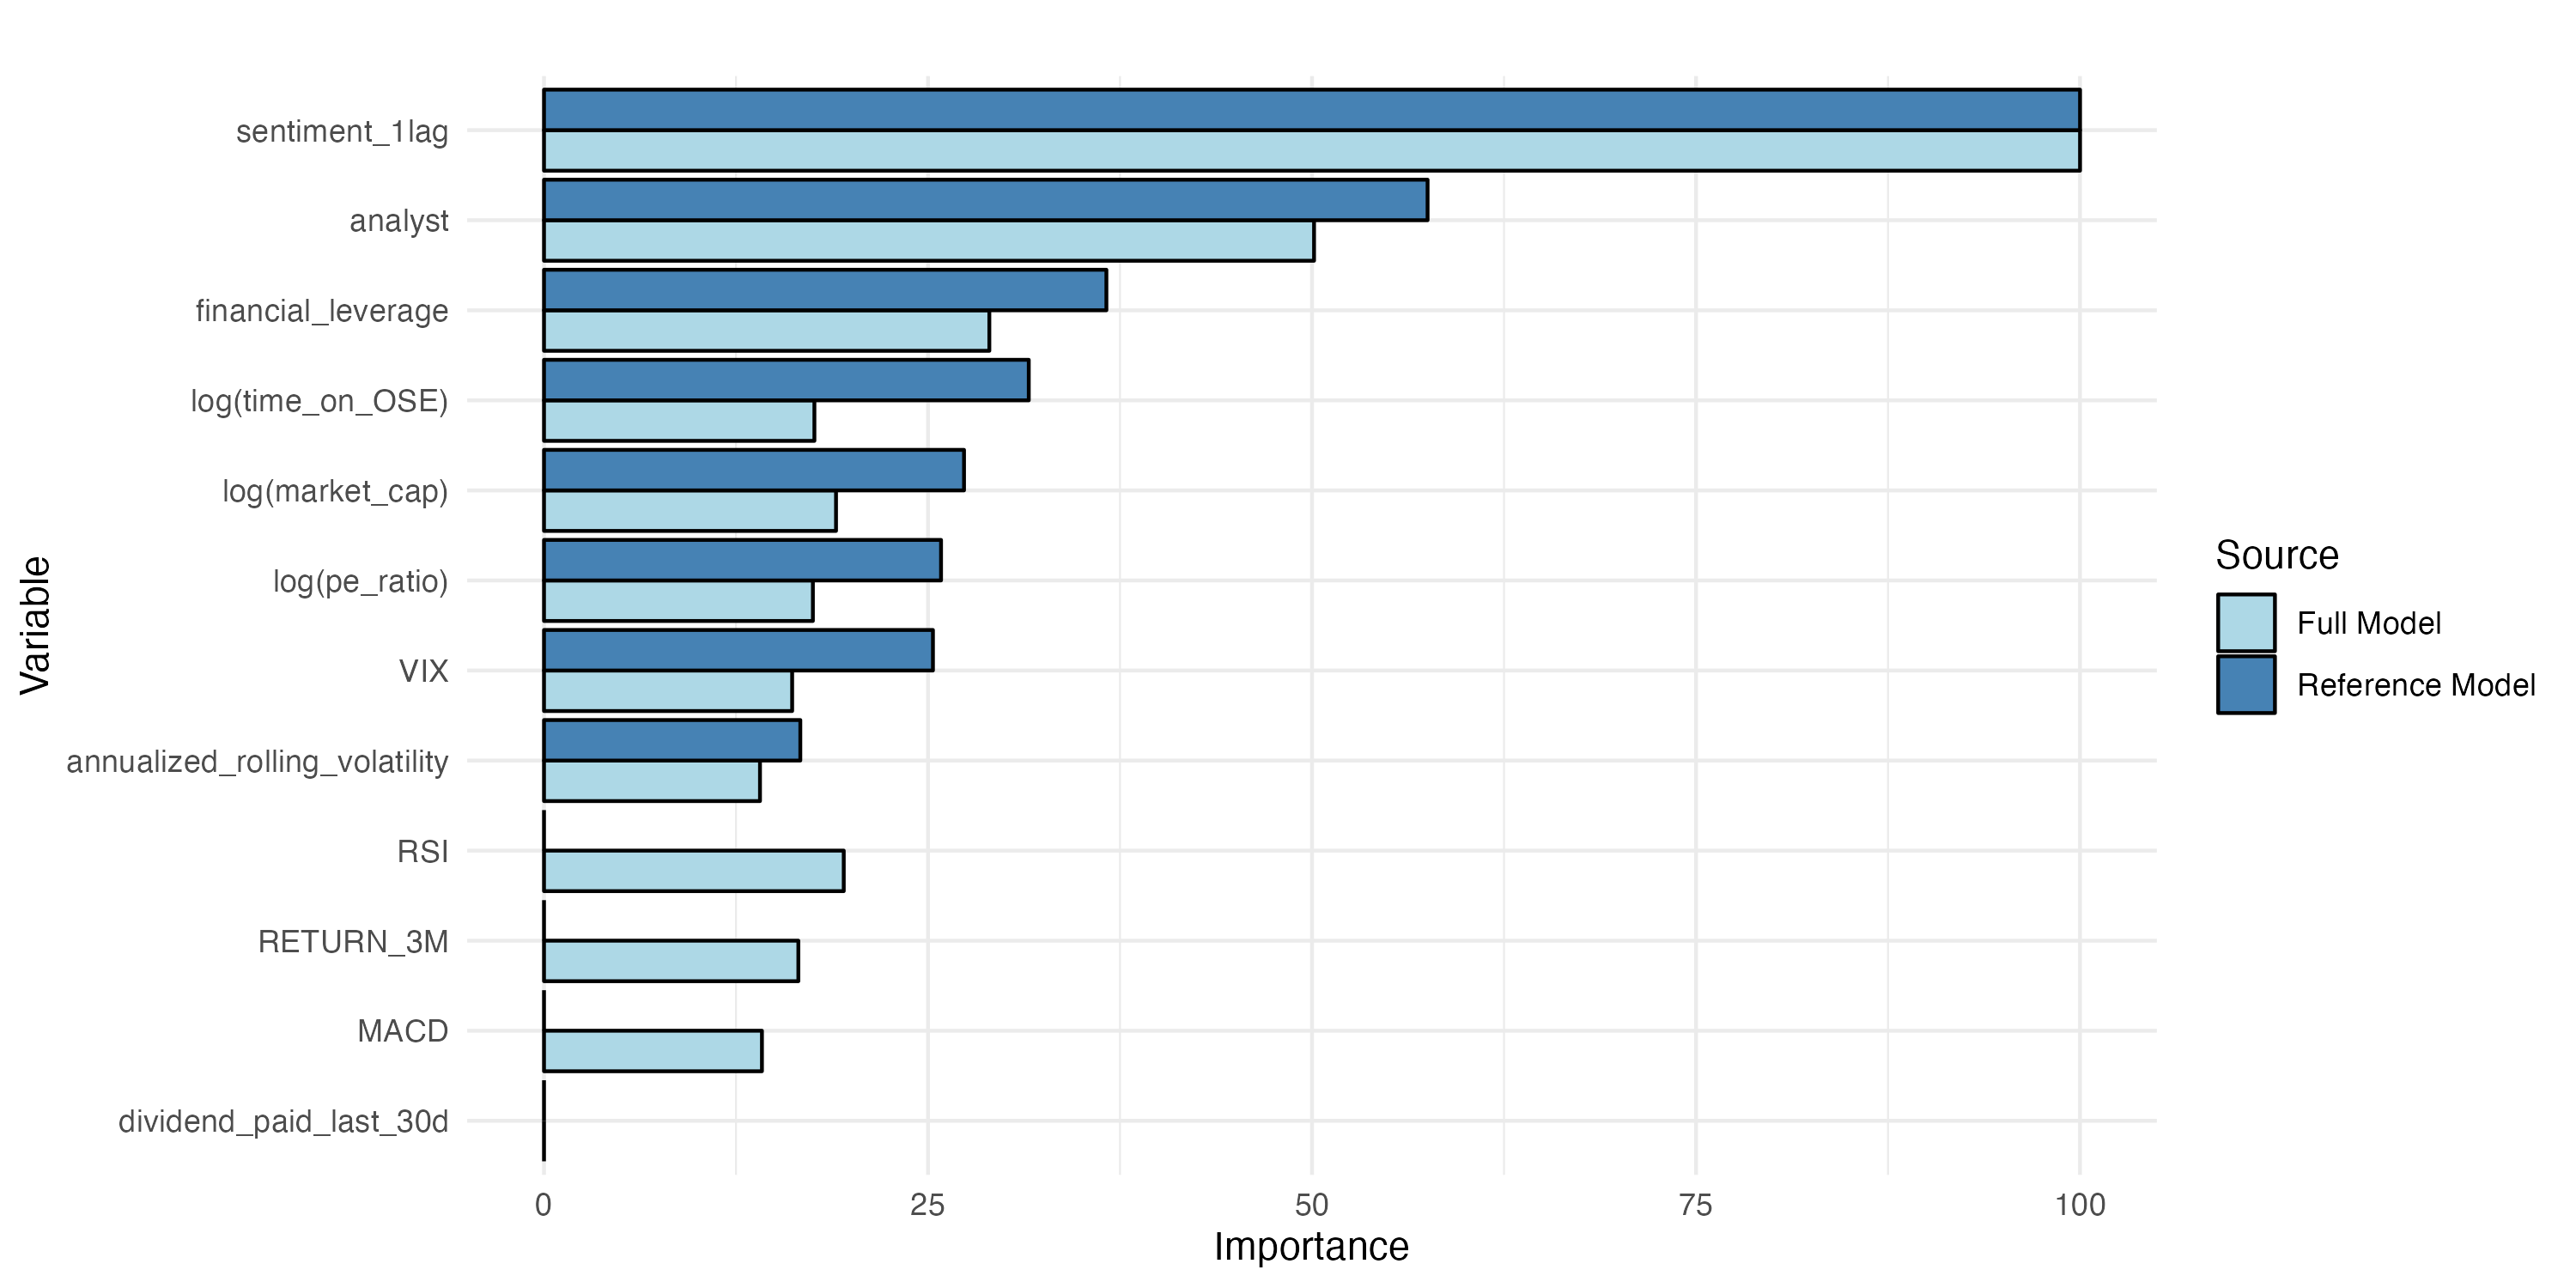
\includegraphics[width=1\textwidth]{Images/variable_imp.png}
    \caption{XGBoost Variable Importance}
    \label{fig:varImp}
\end{figure}

Figure \ref{fig:varImp} tells us that the most important factor in determining textual sentiment is the lagged value for said sentiment. This shows that the attitude towards a given stock is sticky, as the sentiment report in \(t-1\) seems to highly correlate with the sentiment of a report in \(t\). We also find that the investment bank an analyst works for has a lot of impact on the sentiment, which is most likely a result of varying internal guidelines in a given company. The variables continue to be the most important even after we introduce the trend indicators in the full model. This aligns with the assumptions of sticky attitudes and seems to be essential if we want to predict the numerical value of sentiment.

After the lagged sentiment and investment bank we notice a significant fall-off in importance. The financial leverage of a given company is deemed to be the third most important variable in this model. High leverage can signal a greater risk of default or financial distress, which in turn negatively impacts stock prices (\cite{cai2011leverage}), potentially causing negative ERR sentiment. Conversely, manageable leverage often indicates a stable financial position as it can increase returns, likely eliciting positive sentiments in ERRs. 

Variables such as the logarithm of companies' P/E-ratio, market capitalization and time on OSE seem to have a significant impact on prediction, albeit less than the previously mentioned metrics. These variables describe a wide array of company attributes, such as earnings, valuation of equity and its tenure of being a publicly traded company. It is reasonable to assume that these are factors analysts take into account when determining the future performance of a stock. The volatility of a stock and the VIX are the variables which are deemed to be least important for prediction. This can be attributed to the fact that analysts use a six-to-twelve month time-frame when judging target prices. Due to the law of large numbers they may assume that these metrics of uncertainty will even out over time, given that their expected value is estimated to be 0. Recent dividend payout seems to have no impact on sentiment, which could be attributed to effective expectation management from the companies paying out dividends.

When looking at the \textit{Full Model}, we see a shift in the importance of certain variables. RSI is the fourth most important variable, right below financial leverage. This suggests that market movements in the last 14 trading days account for as much predictive power as the leverage of a company. In addition to this, the MACD and three-month return seems to be comparable to the market capitalization and P/E-ratio of a company. Although we cannot conclude that these trend indicators capture the predictive effects, it seems like the textual sentiment in ERRs is affected by market movements in the period leading up to the release of a report. When combined with the fact that the full model has a lower error when predicting new observations than the reference model, it adds up to a conclusion indicating that these market indicators do impact the textual sentiment in the ERRs we have analyzed.

% Either write a summary of these finding, or add to the discussion what can be concluded based on these finding. For example, it is important that we adress the error margins specifically, and how they show, together with the information gathered from the inference sections that our models do not account for all the variance in sentiment (nor should we expect them to!)